In the following hierarchical Bayesian modeling is introduced as a tool for distinguishing and handling uncertainty in codified models of the form \cref{eq:ICASP:EmpiricalRelation}.
% MOTIVATION
The aim of this section is to establish a Bayesian model and updating strategy for the following experimental situation.
% EXPERIMENTAL SITUATION
The compressive strength is measured for a number of clay block masonry specimens.
Specimens can be grouped according to the ensembles of brick units and mortar that were used for their construction.
% ENSEMBLES
Here ensembles of clay bricks are characterized by the same ingredients used and the same manufacturing procedure.
Similarly in every ensemble of mortar samples identical constituents were used for mixing.
% MATERIAL HETEROGENEITY
In this modeling approach material heterogeneity is accounted for by distinguishing between brick and mortar samples used in constructing the masonry wall systems.
% THE GOAL
The final goal is the assessment and prediction of the compressive capacity of structural masonry by utilizing system- and component level information.

\subsection{Aleatory model}
% ALEATORY MODEL
Within an ensemble of masonry wall specimens, the compressive strength of the masonry wall is represented as a random variable
\begin{equation} \label{eq:ICASP:ProbabilisticInterpretation}
  F_w = k F_b^\alpha F_m^\beta.
\end{equation}
% RELATION TO CODE & COEFFICIENTS
This is a probabilistic extension of the codified model in \cref{eq:ICASP:EmpiricalRelation}.
We remark that the coefficients \((k,\alpha,\beta)\) of the relation \cref{eq:ICASP:ProbabilisticInterpretation} are not immediately identified with the ones of \cref{eq:ICASP:EmpiricalRelation}.
\par % COMPONENTS
The compressive strengths of the bricks and the mortar are modeled as lognormal random variables \(F_b \sim \mathcal{LN}(f_b \cond \mu_b,\sigma_b^2)\) and \(F_m \sim \mathcal{LN}(f_m \cond \mu_m,\sigma_m^2)\).
Their distributions are determined by hyperparameters \(\bm{\theta}_b = (\mu_b,\sigma_b)\) and \(\bm{\theta}_m = (\mu_m,\sigma_m)\) that are the mean and standard deviation of \(\log(F_b)\) and \(\log(F_m)\), respectively.
% DISTRIBUTION
Consequently the masonry wall compressive strength in \cref{eq:ICASP:ProbabilisticInterpretation} is a random variable that follows a lognormal distribution
\begin{subequations} \label{eq:ICASP:AleatoryUncertainty}
  \begin{align}
    F_w &\sim \mathcal{LN} \left( f_w \cond \mu_w,\sigma_w^2 \right), \label{eq:ICASP:AleatoryUncertainty:F} \\
    \text{with} \;\, \mu_w &= \alpha \mu_b + \beta \mu_m + \log k, \label{eq:ICASP:AleatoryUncertainty:Mu} \\
    \text{and} \;\, \sigma_w^2 &= \alpha^2 \sigma_b^2 + \beta^2 \sigma_m^2. \label{eq:ICASP:AleatoryUncertainty:Sigma}
  \end{align}
\end{subequations}
% INTERPRETATION
The distribution \cref{eq:ICASP:AleatoryUncertainty:F} represents the variability, i.e.\ the frequency distribution, of the masonry compressive strengths within the population of specimens.
It is parametrized by hyperparameters \(\bm{\theta}_w = (\mu_w,\sigma_w)\) that are determined by the statistical properties of component populations due to \cref{eq:ICASP:AleatoryUncertainty:Mu,eq:ICASP:AleatoryUncertainty:Sigma}.
\par % STATISTICAL PROPERTIES
The mean value and the variance of the distribution \(\mathcal{LN} \left( f_w \cond \mu_w,\sigma_w^2 \right)\) in \cref{eq:ICASP:AleatoryUncertainty} are simply given as
\(\mathds{E}[F_w] = \exp(\mu_w + \sigma_w^2/2)\) and \(\textrm{Var}[F_w] = (\exp(\sigma_w^2)-1) \exp(2\mu_w+\sigma_w^2)\), respectively.
The \(\unit[5]{\%}\)-quantile of  \(\mathcal{LN} \left( f_w \cond \mu_w,\sigma_w^2 \right)\), e.g.\ for comparison with \cref{eq:ICASP:EmpiricalRelation}, follows as \(Q_{w,\unit[5]{\%}} = \exp(\mu_w-1.645 \sigma_w)\).

\subsection{Epistemic model}
% EPISTEMIC UNCERTAINTY
If the coefficients \((k,\alpha,\beta)\) of \cref{eq:ICASP:ProbabilisticInterpretation,eq:ICASP:AleatoryUncertainty} are not perfectly known,
one can represent their epistemic uncertainty as prior random variables \((K,A,B) \sim \pi(k,\alpha,\beta)\).
% BETA = 1-ALPHA
In the following we will confine the analysis to the case \(\beta = 1-\alpha\).
% INDEPENDENT PRIOR
We consider mutually independent prior random variables
\begin{equation} \label{eq:ICASP:EpistemicUncertainty}
  K \sim \pi(k), \quad A \sim \pi(\alpha).
\end{equation}
Their joint prior uncertainty \(\pi(k,\alpha) = \pi(k) \, \pi(\alpha)\) can be reduced by Bayesian data analysis of experimental measurements.
% OUTLOOK
In the following two different updating approaches are outlined for experimental situations where the assumption of known hyperparameters,
i.e.\ the distributional parameters of the ensembles of masonry wall components, is either justified or rather unfounded.

\subsection{Known hyperparameters}
% BATCHES OF EXPERIMENTS
Let us consider experiments of the following type.
In each batch of experiments \(i=1,\ldots,n\) the masonry compressive strength \(f_{w,ij}\) is measured for a number of different specimens \(j=1,\ldots,J_i\) from an ensemble.
We use \(\tuple{f_{w,ij}} = (f_{w,11},\ldots,f_{w,nJ_n})\) to denote the set of these measurements.
The hyperparameters \(\bm{\theta}_{b,i}\) and \(\bm{\theta}_{m,i}\) are measured for the bricks and the mortar used in experiment \(i\), too.
This can be accomplished by a statistical analysis of data \(\tuple{f_{b,ik}} = (f_{b,11},\ldots,f_{b,nK_n})\) and \(\tuple{f_{m,il}} = (f_{m,11},\ldots,f_{m,nK_n})\) with \(k=1,\ldots,K_i\) and \(l=1,\ldots,L_i\).
These data must be numerous and they must be observed for the ensembles of brick units and mortar used.
% BAYESIAN MODEL
The Bayesian multilevel model for this scenario can be written as
\begin{subequations} \label{eq:ICASP:Known:BPN}
  \begin{align}
    (F_{w,ij} \cond k,\alpha) &\sim \pi(f_{w,ij} \cond k,\alpha), \label{eq:ICASP:Known:BPN:Aleatory} \\
    (K,A) &\sim \pi(k) \, \pi(\alpha). \label{eq:ICASP:Known:BPN:Epistemic}
  \end{align}
\end{subequations}
Here the conditional distributions \cref{eq:ICASP:Known:BPN:Aleatory} are given by \cref{eq:ICASP:AleatoryUncertainty}, where batch-specific knowns \(\bm{\theta}_{b,i}\) and \(\bm{\theta}_{b,i}\) are plugged in.
The epistemic prior uncertainty of the coefficients \((k,\alpha)\) is encoded in \cref{eq:ICASP:Known:BPN:Epistemic}.
% (CONDITIONAL) INDEPENDENCE
As long as not indicated otherwise, all random variables in \cref{eq:ICASP:Known:BPN} are assumed to be (conditionally) independent.
% DAG
A directed acyclic graph (DAG) as in \cref{fig:ICASP:DAG:1} serves as an intuitive visualization of the model \cref{eq:ICASP:Known:BPN}.
\begin{figure}[htbp]
  \centering
  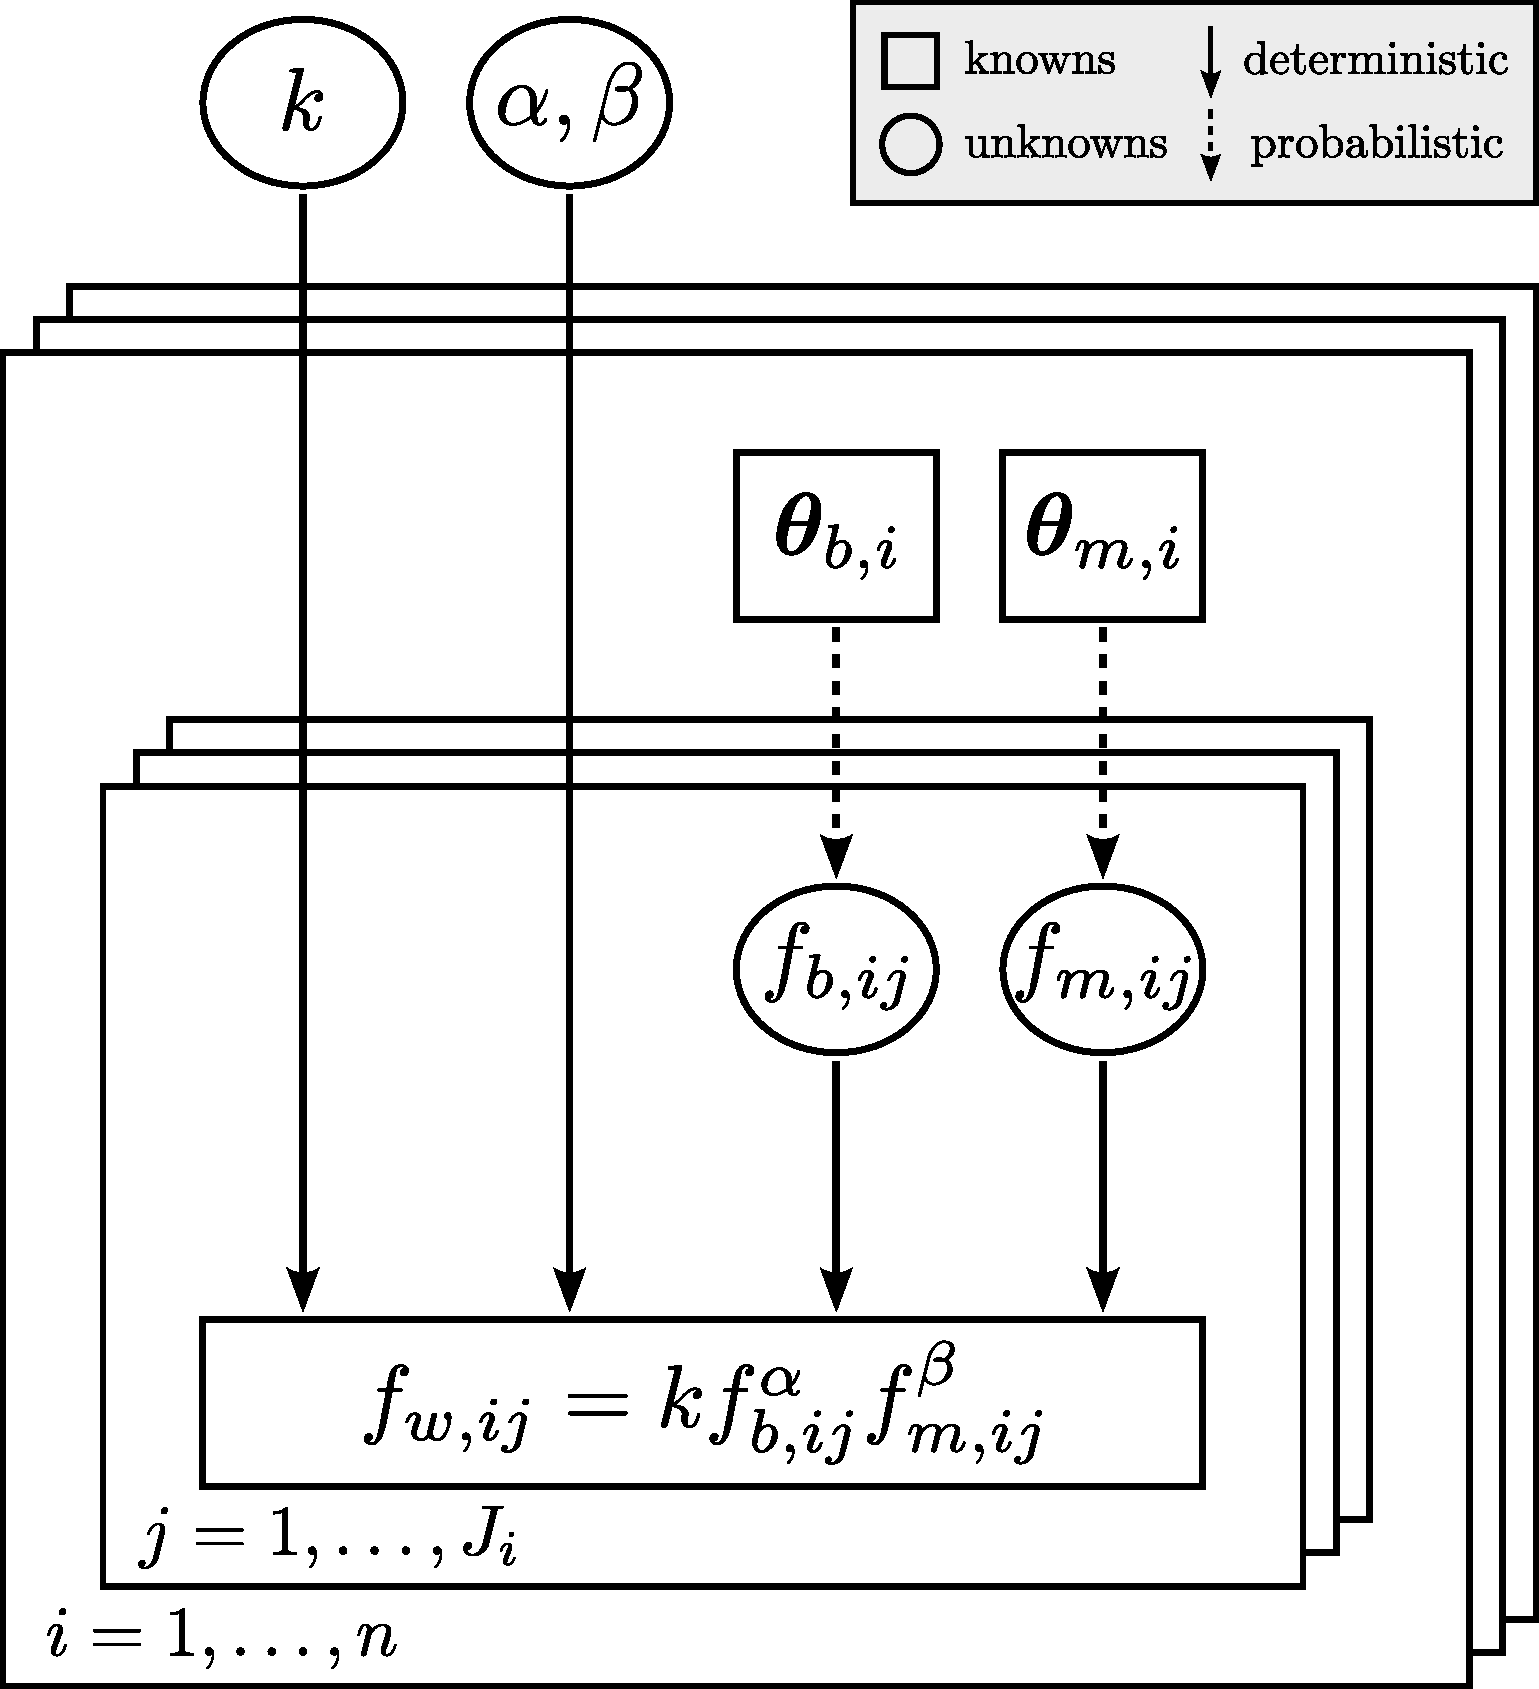
\includegraphics[width=\ICASPdagWidth]{fig_ICASP_DAG1}
  \caption[Known hyperparameters]{Known hyperparameters.
           Nodes symbolize known (\(\vcenter{\hbox{\protect
\includegraphics[height=1.2ex]{fig_Square}}}\))
           or unknown (\(\vcenter{\hbox{\protect
\includegraphics[height=1.3ex]{fig_Circle}}}\)) quantities.
           Arrows represent deterministic (\(\vcenter{\hbox{\protect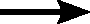
\includegraphics[height=1.0ex]{fig_Solid}}}\))
           or probabilistic (\(\vcenter{\hbox{\protect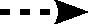
\includegraphics[height=1.0ex]{fig_Dashed}}}\)) relations.
          }
  \label{fig:ICASP:DAG:1}
\end{figure}
\par % POSTERIOR DISTRIBUTION
As usual, Bayesian updating is accomplished by conditioning the prior distribution \(\pi(k,\alpha) = \pi(k) \, \pi(\alpha)\) on the acquired data \(\tuple{f_{w,ij}}\).
One obtains
\begin{equation} \label{eq:ICASP:Known:Posterior}
  \pi(k,\alpha \cond \tuple{f_{w,ij}}) \propto \pi(k) \, \pi(\alpha) \, \prod\limits_{i=1}^n \prod\limits_{j=1}^{J_i} \pi(f_{w,ij} \cond k,\alpha).
\end{equation}
Note that \cref{eq:ICASP:Known:Posterior} is based on exact values the hyperparameters \(\bm{\theta}_{b,i}\) and \(\bm{\theta}_{m,i}\) for every batch \(i\).

\subsection{Unknown hyperparameters}
% RESTRICTIVE ASSUMPTION
The requirement of known hyperparameters \(\bm{\theta}_{b,i}\) and \(\bm{\theta}_{m,i}\) restricts the applicability model \cref{eq:ICASP:Known:BPN} to situations that are rarely met in practice.
Therefore we consider the situation when only prior knowledge \(\pi(\bm{\theta}_{b,i},\bm{\theta}_{m,i}) = \pi(\bm{\theta}_{b,i}) \, \pi(\bm{\theta}_{m,i})\) about the hyperparameters is available.
Additionally in each batch of experiments \(i\) a variable number of measurements \(f_{b,ik}\) and \(f_{m,il}\) for \(k=1,\ldots,K_i\) and \(l=1,\ldots,L_i\)
are taken of the brick unit and the mortar compressive strength, respectively.
% BAYESIAN MODEL
The corresponding hierarchical Bayesian model reads
\begin{subequations} \label{eq:ICASP:Unknown:BPN}
  \begin{align}
    (F_{w,ij} \cond k,\alpha,\bm{\theta}_{b,i},\bm{\theta}_{m,i}) &\sim \pi(f_{w,ij} \cond k,\alpha,\bm{\theta}_{b,i},\bm{\theta}_{m,i}), \nonumber \\
    (F_{b,ik} \cond \bm{\theta}_{b,i}) &\sim \pi(f_{b,ik} \cond \bm{\theta}_{b,i}), \label{eq:ICASP:Unknown:BPN:Aleatory} \\
    (F_{m,il} \cond \bm{\theta}_{m,i}) &\sim \pi(f_{m,il} \cond \bm{\theta}_{m,i}), \nonumber \\[1ex]
    \begin{split}
      (\bm{\Theta}_{b,i},\bm{\Theta}_{m,i}) &\sim \pi(\bm{\theta}_{b,i}) \, \pi(\bm{\theta}_{m,i}), \\
      (K,A) &\sim \pi(k) \, \pi(\alpha). \label{eq:ICASP:Unknown:BPN:Epistemic}
    \end{split}
  \end{align}
\end{subequations}
While \cref{eq:ICASP:Unknown:BPN:Aleatory} summarizes the aleatory uncertainties, \cref{eq:ICASP:Unknown:BPN:Epistemic} contains the epistemic uncertainties.
% DAG
The model \cref{eq:ICASP:Unknown:BPN} is visualized as the DAG in \cref{fig:ICASP:DAG:2}.
% HIDDEN VARIABLES
We remark that the observations \(\tuple{f_{b,ik}}\) and \(\tuple{f_{m,il}}\) inform about the statistical properties \(\bm{\theta}_{b,i}\) and \(\bm{\theta}_{m,i}\) of the component ensembles. 
This way they give information about the unobservable properties of the brick and mortar samples used for constructing the masonry wall \(i\).
\begin{figure}[htbp]
  \centering
  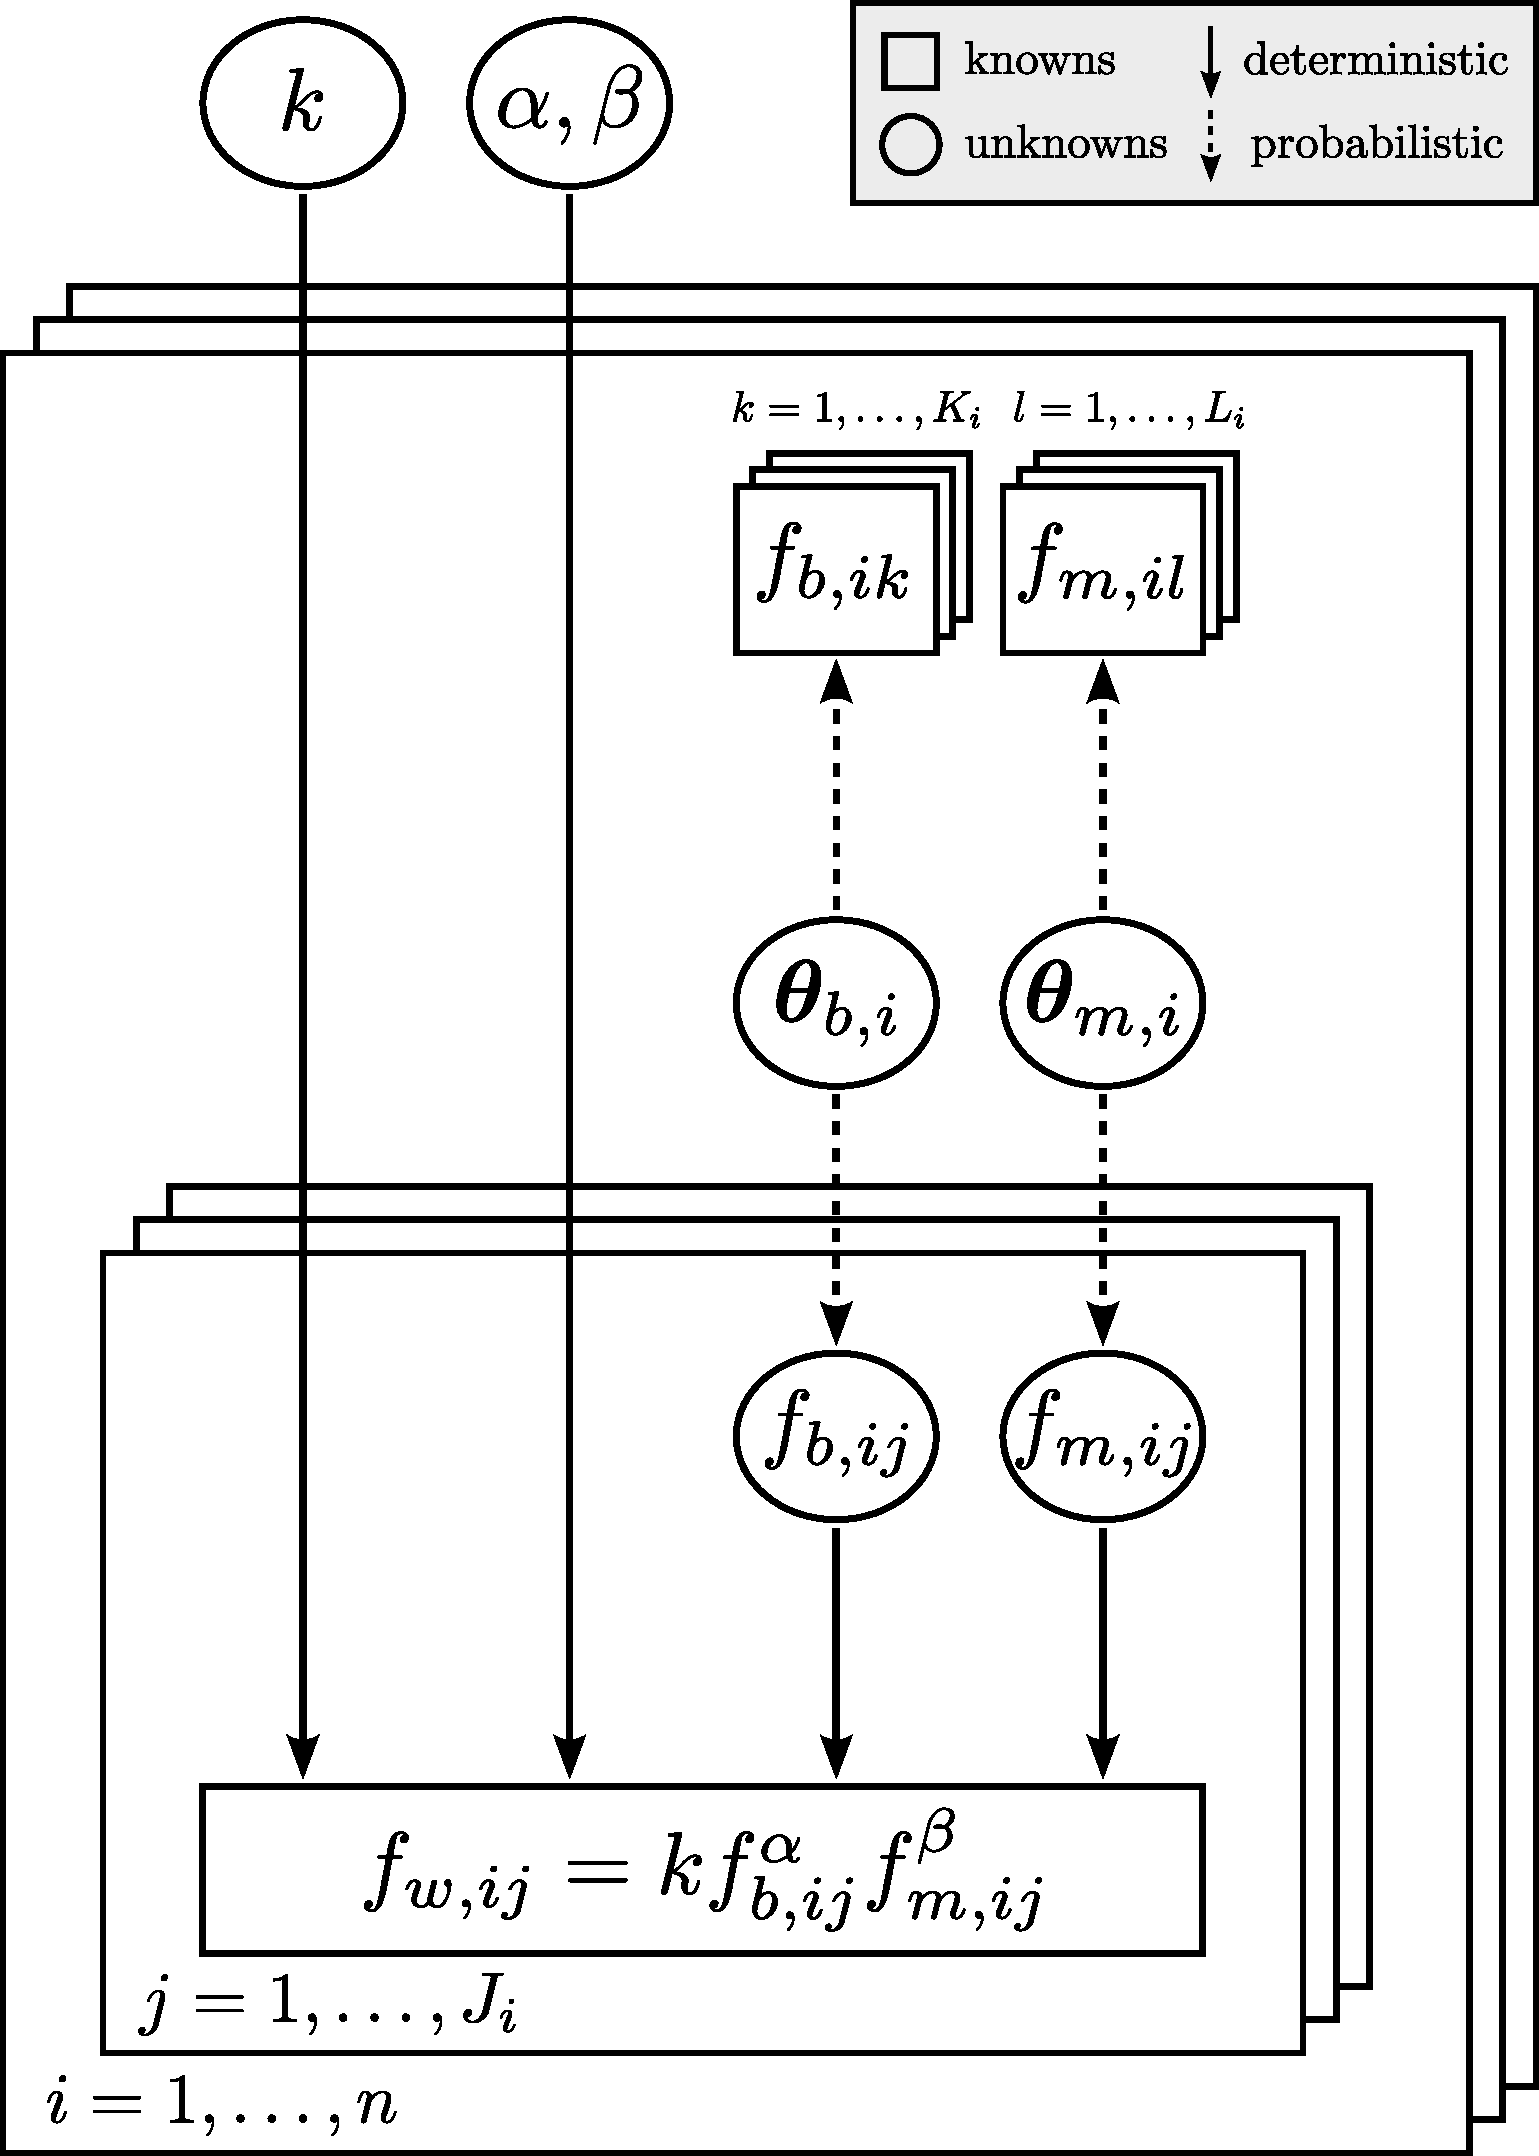
\includegraphics[width=\ICASPdagWidth]{fig_ICASP_DAG2}
  \caption[Unknown hyperparameters]{Unknown hyperparameters.
           The batch-specific hyperparameters \(\bm{\theta}_{b,i}\) and \(\bm{\theta}_{m,i}\) are unknown.
           They can be inferred from the data \(\tuple{f_{b,ik}}\) and \(\tuple{f_{m,il}}\).
          }
  \label{fig:ICASP:DAG:2}
\end{figure}
\par % POSTERIOR DISTRIBUTION
Bayesian analysis proceeds by updating the joint prior \(\pi(k,\alpha,\tuple{\bm{\theta}_{b,i}},\tuple{\bm{\theta}_{m,i}}) = \pi(k) \, \pi(\alpha) \, \prod_{i=1}^n \pi(\bm{\theta}_{b,i}) \, \pi(\bm{\theta}_{m,i})\).
Conditioned on the data \((\tuple{f_{w,ij}},\tuple{f_{b,ik}},\tuple{f_{m,il}})\) one obtains for the joint posterior
\begin{equation} \label{eq:ICASP:Unknown:Posterior}
  \begin{aligned}
    \pi(k,\alpha,\tuple{\bm{\theta}_{b,i}},\tuple{\bm{\theta}_{m,i}} \cond \tuple{f_{w,ij}},\tuple{f_{b,ik}},\tuple{f_{m,il}})
    \propto \pi(k) \, \pi(\alpha) \, \prod\limits_{i=1}^n \pi(\bm{\theta}_{b,i}) \, \pi(\bm{\theta}_{m,i}) \\
    \cdot \;\, \prod\limits_{j=1}^{J_i} \pi(f_{w,ij} \cond k,\alpha,\bm{\theta}_{b,i},\bm{\theta}_{m,i})
    \prod\limits_{k=1}^{K_i} \pi(f_{b,ik} \cond \bm{\theta}_{b,i}) \, \prod\limits_{l=1}^{L_i} \pi(f_{m,il} \cond \bm{\theta}_{m,i}).
  \end{aligned}
\end{equation}
% MULTILEVEL INFORMATION
Notice that the posterior \cref{eq:ICASP:Unknown:Posterior} gathers information from both system- and component-level data.